\documentclass [10pt,a4paper]{report}

\usepackage[utf8]{inputenc}
\usepackage{graphicx}
\begin{document}

\part{Le Grid5000}
	\chapter{Présentation du Grid5000}
Le Grid5000 est une grille informatique destiné à la recherche scientifique. Le projet a vu le jour en 2003 et a pour but de promouvoir la recherche sur les grilles informatiques en France. Le projet est aujourd'hui composé de 1200 noeuds répartis sur 9 sites différents situés en France et au Luxembourg et interconnectés avec le réseau Réseau National de télécommunications pour la Technologie l'Enseignement et la Recherche (RENATER). L'objectif du Grid5000 est de permettre aux scientifiques d'effectuer des expériences dans le domaine des systèmes informatiques et des réseaux distribuées dans un environnement hétèrogene aussi proche de la réalité que possible.

	\begin{figure}[!h]
		\centering
   		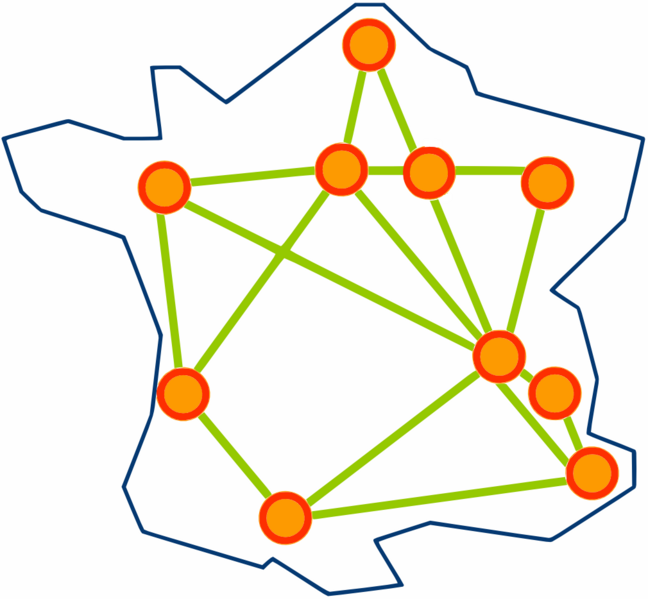
\includegraphics[width=5cm,height=5cm]{map.png}
   		\caption{Localisation des différents sites du Grid5000}
    	\label{fig:map}
	\end{figure} 

Le Grid5000 est donc compsé de plusieurs sites distincts mais l'organisation au sein de chaque site est la même. Chaque site est composé d'un ou plusieurs clusters, c'est à dire un ensemble de machine homogène, par exemple le site de Nancy héberge deux clusters Griffon et Graphene. A l'intérieur de chaque cluster se trouve des ordinateurs aussi appelés "nodes" ou "noeuds". Il existe deux types de nodes : les noeuds de services et les noeuds de travail. Les noeuds de services servent à l'administration des machines situées dans le cluster mais certains noeuds de services appelés "frontends" sont utilisés par les utilisateurs pour l'accès aux différents sites grâce au protocole ssh, la réservation de noeuds et le déploiment. Les "frontends" permettent aussi aux administrateurs d'accéder au hôtes virtuels et aux services d'administration.

\begin{figure}[!h]
		\centering
   		\includegraphics[width=5cm,height=5cm]{griffon.jpeg}
   		\caption{Un des clusters de Nancy : Griffon}
    	\label{fig:griffon}
	\end{figure}
	
	\chapter{Les outils du Grid5000}
		Le Grid5000 est composé de plusieurs services: une partie ces services ont été développés uniquement pour ce projet comme par exemple Kadeploy3 qui a été developpé par l'INRIA Nancy - Grand Est; les autressont des serivices standard utilisés sur les systèmes Unix.  
		\section{OAR}	
		\section{Kadeploy3}
		\section{Taktuk}
		\section{Kavlan}
		\section{Les autres outils}
		
\end{document}